\lhead{\textbf{Basic Algorithms, Fall 2024 \\ CSCI-UA.0310-001}}
\chead{\Large{\textbf{Homework 9}}}
\def\lc{\left\lceil}   
\def\rc{\right\rceil}
\rhead{\textbf{Instructor: Rotem Oshman \\ Name: Ishan Pranav}}
\runningheadrule
\firstpageheadrule
\cfoot{}
\stepcounter{subsection}
\subsection*{References}
Collaborated with Crystal Huang.
\subsection{Sum of degrees}
Prove that in any undirected graph, 
the sum of the degrees of all the vertices is an even number. Recall that the degree of each vertex is the number of edges that include it. For example, in Figure~\ref{fig:box} node $B$ has degree $3$ and node $D$ has degree $2$.

\begin{figure}[htb]
    \centering
    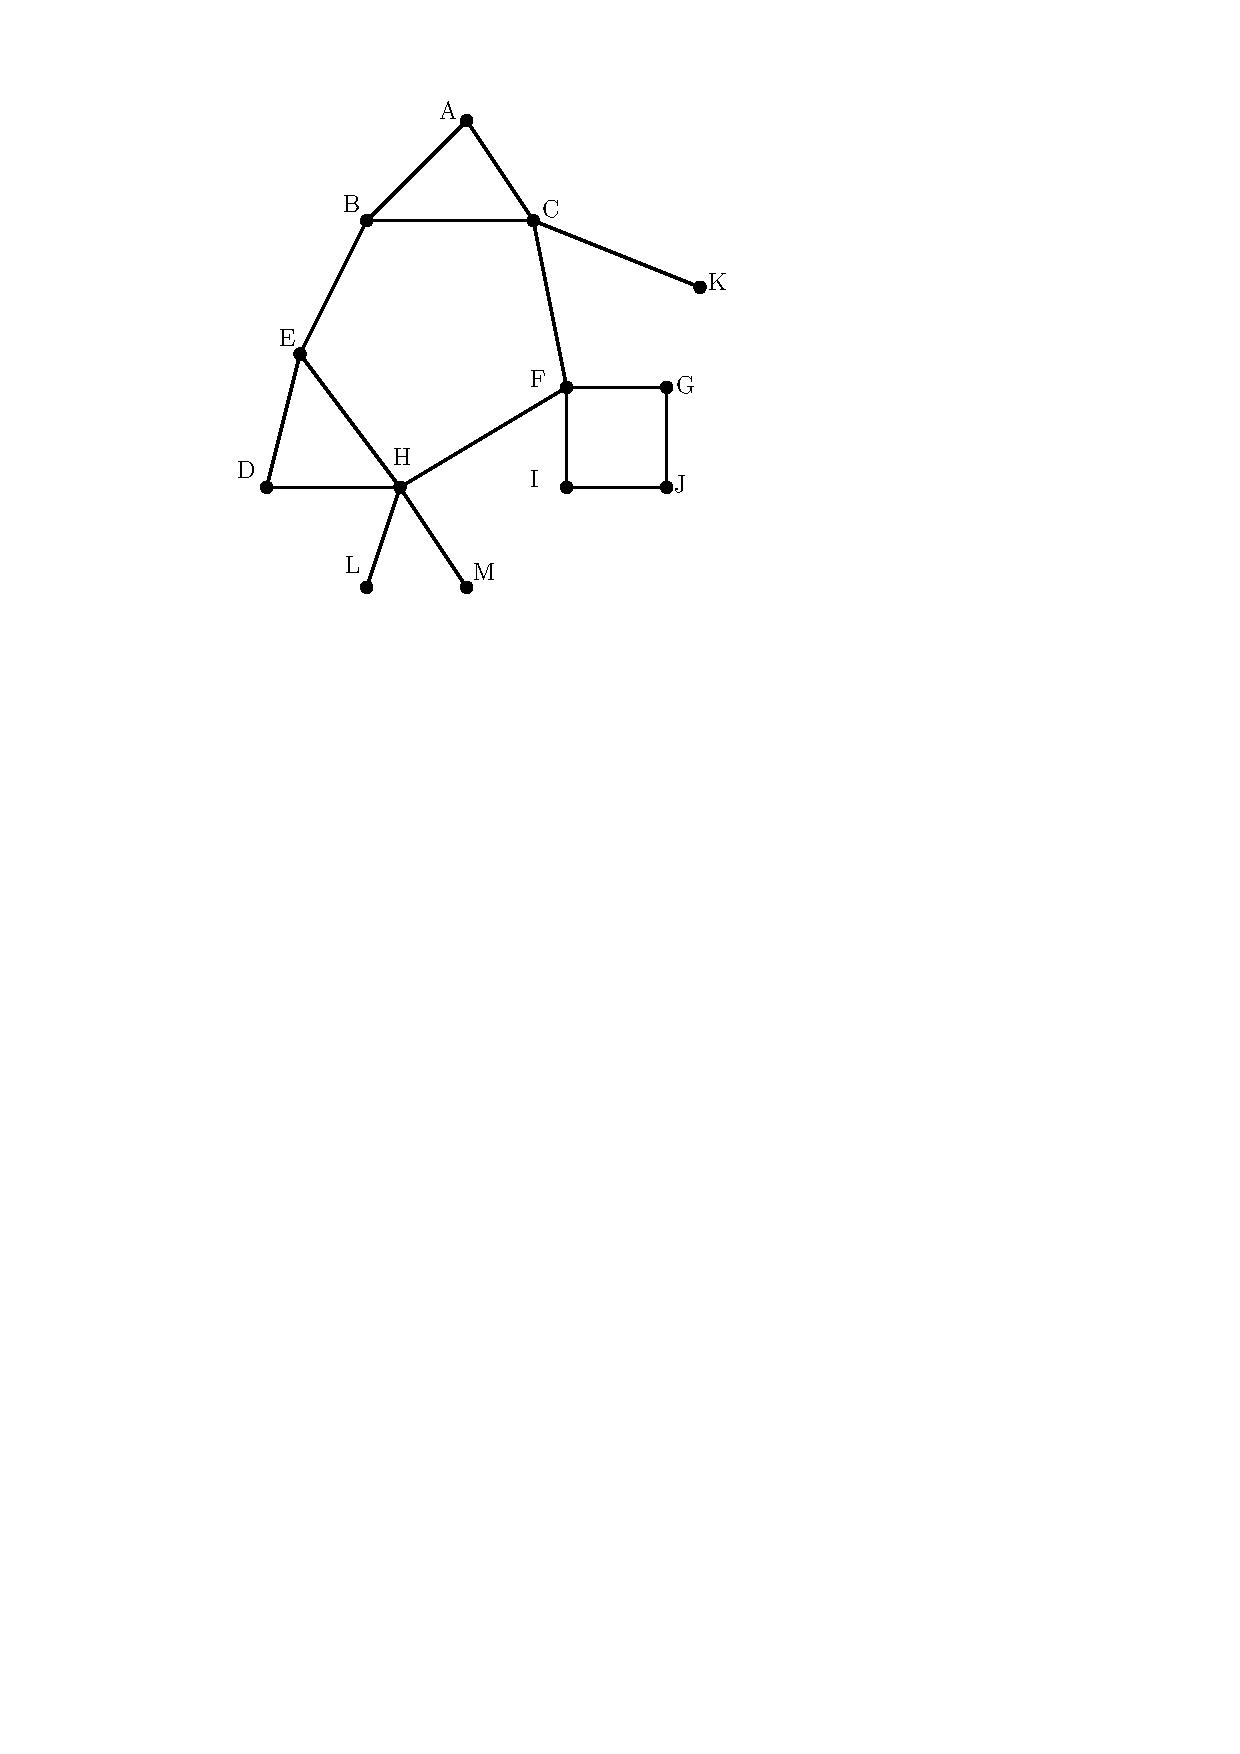
\includegraphics[width=0.4\textwidth]{images/BFS.pdf}
    \caption{An example graph}
    \label{fig:box}
\end{figure}
\begin{solution}
\textit{Claim. }Let $G$ be an undirected graph. Then there exists $k\in\mathbb{Z}$ such that \[\sum_{v\in V}{d_G(v)}=2k,\] where $d(v)$ denotes the degree of vertex $v\in V$ in graph $G$.\\

\noindent\textit{Proof. }We can demonstrate the claim by structural induction on $G$.\\

\noindent\textit{Basis. }Consider $G=(V,\emptyset)$. Then there are no edges in $G$, so for all $v\in V$, we have $d_G(v)=0$. Thus \[\sum_{v\in V}{d_G(v)}=\sum_{v\in V}0=0=2\cdot 0,\]
so the claim holds in the base case.\\

\noindent\textit{Hypothesis. }Consider $G=H=(V,E)$ where $E\neq\emptyset$. Assume that the sum of the degrees of all vertices in graph $H$ is even.\\

\noindent\textit{Inductive step. }Consider $G=(V,E\cup\{\{u,v\}\})$ where $u,v\in V$ and $\{u,v\}\notin E$. Observe
\begin{align*}
\sum_{w\in V}{d_H(w)}
&=d_H(u)+d_H(v)+\sum_{w\in V\setminus\{u,v\}}(d_H(w))\\
&=d_H(u)+d_H(v)+\sum_{w\in V\setminus\{u,v\}}(d_G(w))&\textit{since no $w\in V\setminus\{u,v\}$ is in the new edge,}\\
&=(d_G(u)+1)+(d_G(v)+1)+\sum_{w\in V\setminus\{u,v\}}(d_G(w))&\textit{since $u,v\in\{u,v\}$ but $\{u,v\}\notin E$,}\\
&=2+d_G(u)+d_G(v)+\sum_{w\in V\setminus\{u,v\}}(d_G(w))\\
&=2+\sum_{w\in V}(d_G(w))\\
&=2+2k&\textit{by the inductive hypothesis}\\
&=2(k+1)&\textit{thus completing the inductive step.}
\end{align*}
\noindent Hence, by structural induction, the sum of the degrees of all vertices in an undirected graph is even.$~\square$
\end{solution}
\newpage
\subsection{Depth-first search}

\begin{enumerate}
\item 
Consider the graph in Figure~\ref{fig:box2}. Say we begin a DFS traversal starting at node $A$. List the discovery time (i.e., when we mark a node ``gray'') and finishing time (i.e., when we mark a node ``black'') of each vertex (you may assume each successive step in the traversal takes time 1). Assume that the adjacency lists in the representation of the input graph are in alphabetical order.
\begin{figure}[h!]
\centering
    \begin{tikzpicture}[node distance={20mm}, thick,main/.style={circle, thick,draw,font=\sffamily\bfseries}, ar/.style={-{Stealth[scale=1.2]}}]
          \node[main] (1) {$A$}; 
          \node[main] (2) [below left of=1]{$B$};
          \node[main] (3) [below right of=1]{$C$};
          \node[main] (4) [below of=1]{$D$};
          \node[main] (5) [below left of=4]{$E$};
          \node[main] (6) [below right of=4]{$F$};
          \node[main] (7) [below of=4]{$G$};
          \node[main] (8) [below left of=7]{$H$};
          \node[main] (9) [below right of=7]{$I$};
          
          \draw[ar] (1) -- (2);
          \draw[ar] (3) -- (1);
          \draw[ar] (4) -- (3);
          \draw[ar] (2) -- (5);
          \draw[ar] (7) -- (4);
          \draw[ar] (5) -- (7);
          \draw[ar] (5) -- (8);
          \draw[ar] (9) -- (8);
          \draw[ar] (6) -- (9);
          \draw[ar] (3) -- (6);
          \draw[ar] (4) -- (2);
          \draw[ar] (7) -- (6);
          
    \end{tikzpicture}
    \caption{Graph for Question 2.1}
          \label{fig:box2}
\centering
\end{figure}
    \begin{center}
    \begin{tabular}{|c|c|c|c|c|c|c|c|c|c|}
    \hline
         Node & A & B & C & D & E & F & G & H & I\\
         \hline 
         $d$-time & 1 & 2 & 6 & 5 & 3 & 7 & 4 & 9 & 8 \\
         \hline
         $f$-time & 18 & 17 & 13 & 14 & 16 & 12 & 15 & 10 & 11 \\
         \hline
    \end{tabular}
    \end{center}
\begin{solution}
We can step through the depth-first search algorithm, collecting the times of discovery and finishing for each vertex visited. Visiting adjacent vertices in alphabetical order, we obtain the table above.
\end{solution}
\end{enumerate}    
\newpage
\noindent
As in the previous question, for any vertex $a$ in a directed graph $G$, we denote by $a.\mathsf{d} $ the time at which DFS on $G$ discovers (i.e., marks as ``gray'') the vertex $a$. Similarly, denote by $a.\mathsf{f} $ the time at which DFS fully explores (i.e., marks as ``black'') the vertex $a$. Give counterexamples to the following statements:
\begin{enumerate}[start=2]
    \item If a directed graph $G$ contains a path
    from $a$ to $b$, and if $a.\mathsf{d} < b.\mathsf{d}$ in a depth-first search of $G$, then $b$ is a descendant
    of $a$ in the depth-first forest produced.

\begin{solution}
\textit{False claim. }Let $G=(V,E)$ be a directed graph such that for $a,b\in V$, there exists a path $(a,\dots,b)$. If $a.\mathsf{d}<b.\mathsf{d}$ in a depth-first search of $G$, then $b$ is a descendant of $a$ in the depth-first forest produced. We assume, without loss of generality, that adjacency lists are sorted in alphabetical order.

\textit{Counterexample. }Suppose $G=(\{{\rm X},{\rm Y},{\rm Z}\},\{({\rm X},{\rm Y}),({\rm X},{\rm Z}),({\rm Y},{\rm X})\})$.

Note there exists a path $({\rm Y},{\rm X},{\rm Z})$ from vertex Y to vertex Z. First, we visit X, so ${\rm X}.\mathsf{d}=1$. Then, based on our assumption, we visit ${\rm Y}$, so ${\rm Y}.\mathsf{d}=2$. Upon completing ${\rm Y}$, we have ${\rm Y}.\mathsf{f}=3$. Then, we visit ${\rm Z}$, so ${\rm Z}.\mathsf{d}=4$. Upon completing ${\rm Z}$, we have ${\rm Z}.\mathsf{f}=5$. Finally, we complete ${\rm X}$, giving ${\rm X}.\mathsf{f}=6$. Thus, ${\rm Y}.\mathsf{d}<{\rm Z}.\mathsf{d}$.

However, Y is not a descendant of Z. Hence disproven.$~\square$
\end{solution}
\item If a directed graph $G$ contains a path from $a$ to $b$, then any depth-first search must result in $b.\mathsf{d} < a.\mathsf{f}$.
\begin{solution}
\textit{False claim. }Let $G=(V,E)$ be a directed graph such that for $a,b\in V$, there exists a path $(a,\dots,b)$. Then $b.\mathsf{d}<a.\mathsf{f}$ in a depth-first search of $G$. We assume, without loss of generality, that adjacency lists are sorted in alphabetical order.

\textit{Counterexample. }Suppose $G=(\{{\rm X},{\rm Y},{\rm Z}\},\{({\rm X},{\rm Y}),({\rm X},{\rm Z}),({\rm Y},{\rm X})\})$.

There exists a path $({\rm Y},{\rm X},{\rm Z})$ from vertex Y to vertex Z.

First, we visit X, so ${\rm X}.\mathsf{d}=1$. Then, based on our assumption, we visit ${\rm Y}$, so ${\rm Y}.\mathsf{d}=2$. Upon completing ${\rm Y}$, we have ${\rm Y}.\mathsf{f}=3$. Then, we visit ${\rm Z}$, so ${\rm Z}.\mathsf{d}=4$. Upon completing ${\rm Z}$, we have ${\rm Z}.\mathsf{f}=5$. Finally, we complete ${\rm X}$, giving ${\rm X}.\mathsf{f}=6$. 

Of course, ${\rm Z}.\mathsf{d}\nless{\rm Y}.\mathsf{d}$. Hence disproven.$~\square$
\end{solution}
\end{enumerate}
\newpage
\subsection{2-Colorings}
A \emph{2-coloring} of an undirected graph $G = (V,E)$ assigns each node $v \in V$ a color $v.color \in \{red,green\}$ such that $u.color \neq v.color$ for all $\{u,v\}\in E$. We say the graph $G$ is 2-colorable if such a 2-coloring exists.

\begin{enumerate}
    \item 
    Show that if $G$ is a tree (i.e., connected and acyclic), then there always exists a 2-coloring. How many different 2-colors exist for such a graph?

\begin{solution}

\textbf{Proposition I. }\textit{Claim. }Let $G$ be an undirected graph. If $G$ is a tree, then $G$ is 2-colorable.

\textit{Proof. }Suppose $G$ is a tree. The claim holds vacuously for the trivial graph $G=(\emptyset,\emptyset)$. We can demonstrate the claim for graphs with at least one vertex by structural induction on $G$.

\textit{Basis. }Consider $G=(\{v_0\},E_0)$. Since $G$ is a tree, $G$ is acyclic, and thus $E_0=\emptyset$. Assume, without of loss of generality, that we color the root vertex $v_0$ red. Then $G$ is 2-colorable.

\textit{Hypothesis. }Consider $G=(V,E)$ where $|V|>1$. Assume that $(V,E)$ is 2-colorable.

\textit{Inductive step. }Consider $G=(V',E')$ where $|V'|=|V|+1$. Since $G$ is a non-trivial tree, there exits a leaf $v\in V'$. Separating $v$ from $G$ produces two induced subtrees of $G$: one tree $H$ with $|V|$ vertices, and another with one vertex, $v$.

Since $G$ is a tree, and thus connected, and since $G$ has at least 2 vertices, there exists a single edge $\{u,v\}\in E'$ connecting leaf $v$ to some other vertex $u\in V'$.

Of course, $H$ is the subgraph induced by removing $v$ from $G$, so $H=(V'\setminus\{v\},E'\setminus\{\{u,v\}\})$.

There exists a 2-coloring of $H$ by the inductive hypothesis. In this coloring for $H$, $u$ is either red or green:
\begin{itemize}
\item Suppose $u$ is red. For $G$, we color $v$ green and color each other vertex to match its coloring for $H$.
\item Suppose instead $u$ is green. For $G$, we color $v$ red and color each other vertex to match its coloring for $H$.
\end{itemize}
In both cases, the inductive hypothesis guarantees that the 2-coloring is valid for all vertices $w\in V$ and edges $e\in E$, and it is also valid for edge $\{u,v\}$ (since $u.\mathsf{color}\neq v.\mathsf{color}$), so the 2-coloring is valid for all vertices $w\in V'$ and edges $e\in E'$.

Hence, by structural induction, $G$ is 2-colorable.$~\square$

\textbf{Proposition II. }\textit{Claim. }Let $G$ be a tree. Then there exist two 2-colorings for $G$.

\textit{Proof. }The base case of Proposition I assumes, without loss of generality, that, for all trees $G$, we color the root vertex red. We may instead color the root vertex green to produce a distinct, but equally valid, 2-coloring of $G$. Ergo, there exist two 2-colorings for each tree $G.~\square$
\end{solution}
\newpage
\item 
	Describe how to modify the algorithm for Depth First Search so that it assigns a valid 2-coloring, or returns an error in case none exists. To this end, write a function {\sc TwoColoring-Visit}$(G,u,c)$ that takes a graph $G$, a vertex $u$, and a color $c \in \{red,green\}$ such that the following driver function either assigns a valid 2-coloring and returns $success$, or returns $error$ in case no 2-coloring exists. Your algorithm should assume $G$ to be represented as an adjacency list and run in $O(|V| + |E|)$. 
	
	\begin{code}
		{\sc TwoColoring}$(G)$\\
		\> \For $u \in G.V$ \Do \\
		\> \> $u.color = white$ \\
		\> \For $u \in G.V$ \Do \\
		\> \> \If $u.color \stackrel{?}{=} white$ \Then \\
		\> \> \> $\text{\sc TwoColoring-Visit}(G,u,red)$ \\
		\> \Return $success$ \\
	\end{code}
\begin{solution}
{\sc TwoColoring--Visit}($G,u,c$) with graph $G=(V,E)$, vertex $u\in V$, and color $c\in\{\mathsf{red},\mathsf{green}\}$:

Assign property $u.\mathsf{color}\leftarrow c$.

For each $v\in V$ where $\{u,v\}\in E$, via adjacency list:
\begin{itemize}
\item if $v.\mathsf{color}=\text{white}$, then:
\begin{itemize}
    \item $c'\leftarrow\mathsf{red}$ if $c=\mathsf{green}$; otherwise, $\mathsf{green}$;
    \item perform {\sc TwoColoring--Visit}($G,v,c'$);
\end{itemize}
\item otherwise, if $v.\mathsf{color}=u.\mathsf{color}$, then
\begin{itemize}
    \item throw an exception that cascades up to the parent algorithm, so that {\sc TwoColoring} returns the error condition.
\end{itemize}
\end{itemize}
\textbf{Proposition III. }\textit{Claim. }{\sc TwoColoring} has running time $O(|V|+|E|)$.

\textit{Proof. }{\sc TwoColoring} is a variant of the well-known depth-first search algorithm, which has running time $O(|V|+E|)$. Intuitively, {\sc TwoColoring} visits each vertex, and for each vertex, recursively visits the members of its adjacency list. Each vertex is visited at most once, since once a vertex is no longer colored $\mathsf{white}$, it is no longer considered. The total number of adjacency list entries across all vertices is $2|E|$. Thus the running time is $O(|V|+2|E|)=O(|V|+|E|).~\square$
\end{solution}
\newpage
\item Prove the correctness of your algorithm. More concretely, show (a) that the assigned coloring is always a valid 2-coloring, and (b) if a 2-coloring exists then the algorithm does assign one.
\begin{solution}
\textbf{Proposition IV. }\textit{Claim. }{\sc TwoColoring} always assigns a valid 2-coloring, and, if a 2 coloring exists, {\sc TwoColoring} does assign one.

\textit{Proof. }{\sc TwoColoring} is a variant of the well-known depth-first search algorithm: We can thus produce a ``depth-first search forest'' $F=(V,E)$ by tracing the steps of the algorithm.

Since {\sc TwoColoring} operates on undirected graphs only, for all $\{u,v\}\in E$, either $\{u,v\}$ is a tree edge or a back edge:
\begin{itemize}
    \item Suppose $\{u,v\}$ is a tree edge. From Proposition I, there exists a 2-coloring for any tree. If $\{u,v\}$ is a tree edge, then $v.\mathsf{color}=\mathsf{white}$. By assigning the color of each vertex to be different from its parent's color, {\sc TwoColoring--Visit} preserves the validity of the 2-coloring, as done in the inductive step of Proposition I.
    \item Suppose instead $\{u,v\}$ is a back edge. Recall that a back-edge implies an edge from vertex $u$ to its ancestor vertex $v$. That is, $v.\mathsf{color}\neq\mathsf{white}$.
    
    Note that the ``2-colorable'' property is synonymous with ``bipartite.'' We know that a graph with an odd-length cycle is not bipartite: If there exists an odd-length cycle---for example, $(x,y,x)$---it is impossible to color vertices $x$ and $y$ to satisfy the 2-colorable property.
    
    A back edge $\{u,v\}$ implies a cycle $(v,\dots,u,v)$.
    
    If $u.\mathsf{color}=v.\mathsf{color}$ (where $u.\mathsf{color}\neq\mathsf{white}$ and $v.\mathsf{color}\neq\mathsf{white}$), then, based on the implementation of {\sc TwoColoring--Visit}, there exists an even-length path $(v,\dots,u)$. This implies that the cycle $(v,\dots,u,v)$ is an odd-length cycle, and thus, the graph is not 2-colorable. In this case, the algorithm correctly raises the error condition.

    Otherwise, there is no evidence that the graph is not bipartite, so we continue coloring the unvisited vertices.
\end{itemize}
If a graph is bipartite, then it is 2-colorable. A graph $G$ is bipartite if and only if there exist no odd-length cycles in $G$. The above analysis of the depth-first search forest $F$ indicates that the algorithm produces a correct 2-coloring if one exists, and raises the error condition if there exists an odd-length cycle in $G$. This demonstrates the correctness of the {\sc TwoColoring} algorithm.$~\square$
\end{solution}
\end{enumerate}
